% Created by tikzDevice version 0.12.3.1 on 2022-09-20 14:40:41
% !TEX encoding = UTF-8 Unicode
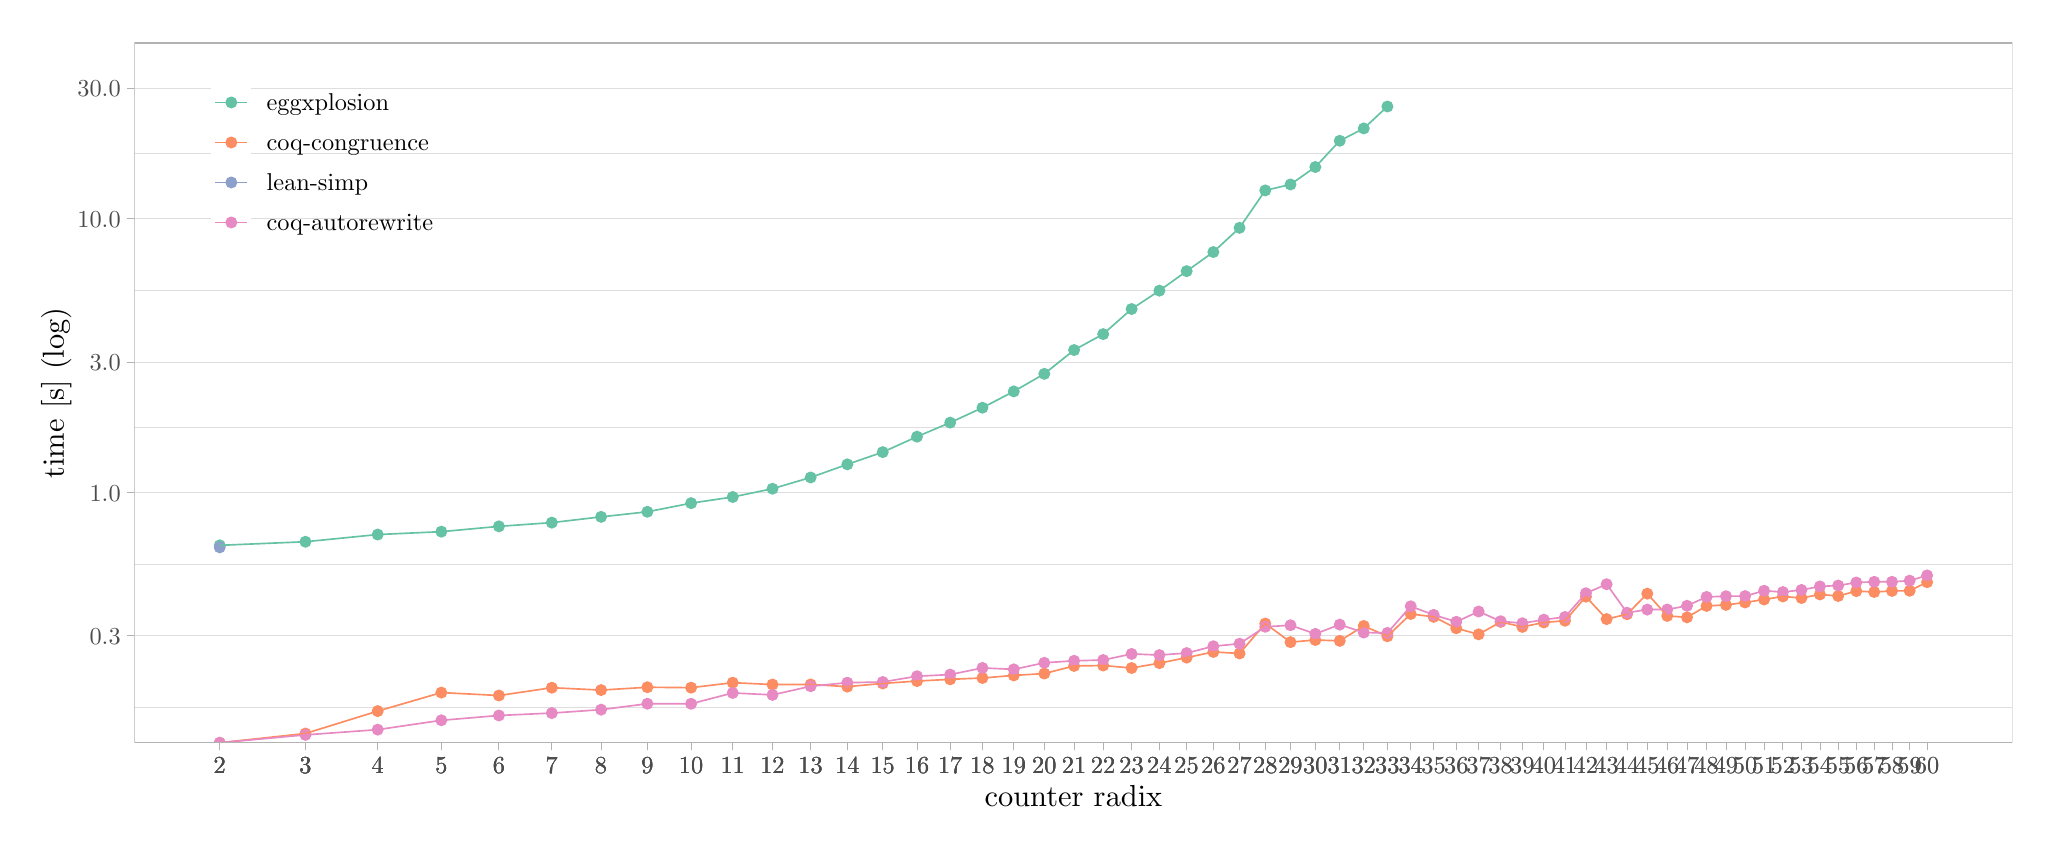
\begin{tikzpicture}[x=1pt,y=1pt]
\definecolor{fillColor}{RGB}{255,255,255}
\path[use as bounding box,fill=fillColor,fill opacity=0.00] (0,0) rectangle (722.70,289.08);
\begin{scope}
\path[clip] (  0.00,  0.00) rectangle (722.70,289.08);
\definecolor{drawColor}{RGB}{255,255,255}
\definecolor{fillColor}{RGB}{255,255,255}

\path[draw=drawColor,line width= 0.6pt,line join=round,line cap=round,fill=fillColor] (  0.00,  0.00) rectangle (722.70,289.08);
\end{scope}
\begin{scope}
\path[clip] ( 38.56, 30.69) rectangle (717.20,283.58);
\definecolor{fillColor}{RGB}{255,255,255}

\path[fill=fillColor] ( 38.56, 30.69) rectangle (717.20,283.58);
\definecolor{drawColor}{gray}{0.87}

\path[draw=drawColor,line width= 0.1pt,line join=round] ( 38.56, 43.44) --
	(717.20, 43.44);

\path[draw=drawColor,line width= 0.1pt,line join=round] ( 38.56, 95.18) --
	(717.20, 95.18);

\path[draw=drawColor,line width= 0.1pt,line join=round] ( 38.56,144.65) --
	(717.20,144.65);

\path[draw=drawColor,line width= 0.1pt,line join=round] ( 38.56,194.12) --
	(717.20,194.12);

\path[draw=drawColor,line width= 0.1pt,line join=round] ( 38.56,243.59) --
	(717.20,243.59);

\path[draw=drawColor,line width= 0.3pt,line join=round] ( 38.56, 69.31) --
	(717.20, 69.31);

\path[draw=drawColor,line width= 0.3pt,line join=round] ( 38.56,121.04) --
	(717.20,121.04);

\path[draw=drawColor,line width= 0.3pt,line join=round] ( 38.56,168.25) --
	(717.20,168.25);

\path[draw=drawColor,line width= 0.3pt,line join=round] ( 38.56,219.99) --
	(717.20,219.99);

\path[draw=drawColor,line width= 0.3pt,line join=round] ( 38.56,267.20) --
	(717.20,267.20);
\definecolor{drawColor}{RGB}{102,194,165}
\definecolor{fillColor}{RGB}{102,194,165}

\path[draw=drawColor,line width= 0.4pt,line join=round,line cap=round,fill=fillColor] ( 69.40,102.02) circle (  1.96);
\definecolor{drawColor}{RGB}{141,160,203}
\definecolor{fillColor}{RGB}{141,160,203}

\path[draw=drawColor,line width= 0.4pt,line join=round,line cap=round,fill=fillColor] ( 69.40,101.29) circle (  1.96);
\definecolor{drawColor}{RGB}{252,141,98}
\definecolor{fillColor}{RGB}{252,141,98}

\path[draw=drawColor,line width= 0.4pt,line join=round,line cap=round,fill=fillColor] ( 69.40, 30.69) circle (  1.96);
\definecolor{drawColor}{RGB}{231,138,195}
\definecolor{fillColor}{RGB}{231,138,195}

\path[draw=drawColor,line width= 0.4pt,line join=round,line cap=round,fill=fillColor] ( 69.40, 30.69) circle (  1.96);
\definecolor{drawColor}{RGB}{102,194,165}
\definecolor{fillColor}{RGB}{102,194,165}

\path[draw=drawColor,line width= 0.4pt,line join=round,line cap=round,fill=fillColor] (100.37,103.32) circle (  1.96);
\definecolor{drawColor}{RGB}{252,141,98}
\definecolor{fillColor}{RGB}{252,141,98}

\path[draw=drawColor,line width= 0.4pt,line join=round,line cap=round,fill=fillColor] (100.37, 34.03) circle (  1.96);
\definecolor{drawColor}{RGB}{231,138,195}
\definecolor{fillColor}{RGB}{231,138,195}

\path[draw=drawColor,line width= 0.4pt,line join=round,line cap=round,fill=fillColor] (100.37, 33.53) circle (  1.96);
\definecolor{drawColor}{RGB}{102,194,165}
\definecolor{fillColor}{RGB}{102,194,165}

\path[draw=drawColor,line width= 0.4pt,line join=round,line cap=round,fill=fillColor] (126.48,105.92) circle (  1.96);
\definecolor{drawColor}{RGB}{252,141,98}
\definecolor{fillColor}{RGB}{252,141,98}

\path[draw=drawColor,line width= 0.4pt,line join=round,line cap=round,fill=fillColor] (126.48, 42.12) circle (  1.96);
\definecolor{drawColor}{RGB}{231,138,195}
\definecolor{fillColor}{RGB}{231,138,195}

\path[draw=drawColor,line width= 0.4pt,line join=round,line cap=round,fill=fillColor] (126.48, 35.42) circle (  1.96);
\definecolor{drawColor}{RGB}{102,194,165}
\definecolor{fillColor}{RGB}{102,194,165}

\path[draw=drawColor,line width= 0.4pt,line join=round,line cap=round,fill=fillColor] (149.48,106.96) circle (  1.96);
\definecolor{drawColor}{RGB}{252,141,98}
\definecolor{fillColor}{RGB}{252,141,98}

\path[draw=drawColor,line width= 0.4pt,line join=round,line cap=round,fill=fillColor] (149.48, 48.81) circle (  1.96);
\definecolor{drawColor}{RGB}{231,138,195}
\definecolor{fillColor}{RGB}{231,138,195}

\path[draw=drawColor,line width= 0.4pt,line join=round,line cap=round,fill=fillColor] (149.48, 38.80) circle (  1.96);
\definecolor{drawColor}{RGB}{102,194,165}
\definecolor{fillColor}{RGB}{102,194,165}

\path[draw=drawColor,line width= 0.4pt,line join=round,line cap=round,fill=fillColor] (170.28,108.88) circle (  1.96);
\definecolor{drawColor}{RGB}{252,141,98}
\definecolor{fillColor}{RGB}{252,141,98}

\path[draw=drawColor,line width= 0.4pt,line join=round,line cap=round,fill=fillColor] (170.28, 47.76) circle (  1.96);
\definecolor{drawColor}{RGB}{231,138,195}
\definecolor{fillColor}{RGB}{231,138,195}

\path[draw=drawColor,line width= 0.4pt,line join=round,line cap=round,fill=fillColor] (170.28, 40.54) circle (  1.96);
\definecolor{drawColor}{RGB}{102,194,165}
\definecolor{fillColor}{RGB}{102,194,165}

\path[draw=drawColor,line width= 0.4pt,line join=round,line cap=round,fill=fillColor] (189.40,110.23) circle (  1.96);
\definecolor{drawColor}{RGB}{252,141,98}
\definecolor{fillColor}{RGB}{252,141,98}

\path[draw=drawColor,line width= 0.4pt,line join=round,line cap=round,fill=fillColor] (189.40, 50.57) circle (  1.96);
\definecolor{drawColor}{RGB}{231,138,195}
\definecolor{fillColor}{RGB}{231,138,195}

\path[draw=drawColor,line width= 0.4pt,line join=round,line cap=round,fill=fillColor] (189.40, 41.41) circle (  1.96);
\definecolor{drawColor}{RGB}{102,194,165}
\definecolor{fillColor}{RGB}{102,194,165}

\path[draw=drawColor,line width= 0.4pt,line join=round,line cap=round,fill=fillColor] (207.20,112.31) circle (  1.96);
\definecolor{drawColor}{RGB}{252,141,98}
\definecolor{fillColor}{RGB}{252,141,98}

\path[draw=drawColor,line width= 0.4pt,line join=round,line cap=round,fill=fillColor] (207.20, 49.72) circle (  1.96);
\definecolor{drawColor}{RGB}{231,138,195}
\definecolor{fillColor}{RGB}{231,138,195}

\path[draw=drawColor,line width= 0.4pt,line join=round,line cap=round,fill=fillColor] (207.20, 42.64) circle (  1.96);
\definecolor{drawColor}{RGB}{102,194,165}
\definecolor{fillColor}{RGB}{102,194,165}

\path[draw=drawColor,line width= 0.4pt,line join=round,line cap=round,fill=fillColor] (223.92,114.14) circle (  1.96);
\definecolor{drawColor}{RGB}{252,141,98}
\definecolor{fillColor}{RGB}{252,141,98}

\path[draw=drawColor,line width= 0.4pt,line join=round,line cap=round,fill=fillColor] (223.92, 50.74) circle (  1.96);
\definecolor{drawColor}{RGB}{231,138,195}
\definecolor{fillColor}{RGB}{231,138,195}

\path[draw=drawColor,line width= 0.4pt,line join=round,line cap=round,fill=fillColor] (223.92, 44.79) circle (  1.96);
\definecolor{drawColor}{RGB}{102,194,165}
\definecolor{fillColor}{RGB}{102,194,165}

\path[draw=drawColor,line width= 0.4pt,line join=round,line cap=round,fill=fillColor] (239.73,117.26) circle (  1.96);
\definecolor{drawColor}{RGB}{252,141,98}
\definecolor{fillColor}{RGB}{252,141,98}

\path[draw=drawColor,line width= 0.4pt,line join=round,line cap=round,fill=fillColor] (239.73, 50.59) circle (  1.96);
\definecolor{drawColor}{RGB}{231,138,195}
\definecolor{fillColor}{RGB}{231,138,195}

\path[draw=drawColor,line width= 0.4pt,line join=round,line cap=round,fill=fillColor] (239.73, 44.77) circle (  1.96);
\definecolor{drawColor}{RGB}{102,194,165}
\definecolor{fillColor}{RGB}{102,194,165}

\path[draw=drawColor,line width= 0.4pt,line join=round,line cap=round,fill=fillColor] (254.77,119.49) circle (  1.96);
\definecolor{drawColor}{RGB}{252,141,98}
\definecolor{fillColor}{RGB}{252,141,98}

\path[draw=drawColor,line width= 0.4pt,line join=round,line cap=round,fill=fillColor] (254.77, 52.39) circle (  1.96);
\definecolor{drawColor}{RGB}{231,138,195}
\definecolor{fillColor}{RGB}{231,138,195}

\path[draw=drawColor,line width= 0.4pt,line join=round,line cap=round,fill=fillColor] (254.77, 48.68) circle (  1.96);
\definecolor{drawColor}{RGB}{102,194,165}
\definecolor{fillColor}{RGB}{102,194,165}

\path[draw=drawColor,line width= 0.4pt,line join=round,line cap=round,fill=fillColor] (269.14,122.48) circle (  1.96);
\definecolor{drawColor}{RGB}{252,141,98}
\definecolor{fillColor}{RGB}{252,141,98}

\path[draw=drawColor,line width= 0.4pt,line join=round,line cap=round,fill=fillColor] (269.14, 51.72) circle (  1.96);
\definecolor{drawColor}{RGB}{231,138,195}
\definecolor{fillColor}{RGB}{231,138,195}

\path[draw=drawColor,line width= 0.4pt,line join=round,line cap=round,fill=fillColor] (269.14, 47.98) circle (  1.96);
\definecolor{drawColor}{RGB}{102,194,165}
\definecolor{fillColor}{RGB}{102,194,165}

\path[draw=drawColor,line width= 0.4pt,line join=round,line cap=round,fill=fillColor] (282.92,126.55) circle (  1.96);
\definecolor{drawColor}{RGB}{252,141,98}
\definecolor{fillColor}{RGB}{252,141,98}

\path[draw=drawColor,line width= 0.4pt,line join=round,line cap=round,fill=fillColor] (282.92, 51.75) circle (  1.96);
\definecolor{drawColor}{RGB}{231,138,195}
\definecolor{fillColor}{RGB}{231,138,195}

\path[draw=drawColor,line width= 0.4pt,line join=round,line cap=round,fill=fillColor] (282.92, 51.10) circle (  1.96);
\definecolor{drawColor}{RGB}{102,194,165}
\definecolor{fillColor}{RGB}{102,194,165}

\path[draw=drawColor,line width= 0.4pt,line join=round,line cap=round,fill=fillColor] (296.18,131.28) circle (  1.96);
\definecolor{drawColor}{RGB}{252,141,98}
\definecolor{fillColor}{RGB}{252,141,98}

\path[draw=drawColor,line width= 0.4pt,line join=round,line cap=round,fill=fillColor] (296.18, 50.96) circle (  1.96);
\definecolor{drawColor}{RGB}{231,138,195}
\definecolor{fillColor}{RGB}{231,138,195}

\path[draw=drawColor,line width= 0.4pt,line join=round,line cap=round,fill=fillColor] (296.18, 52.39) circle (  1.96);
\definecolor{drawColor}{RGB}{102,194,165}
\definecolor{fillColor}{RGB}{102,194,165}

\path[draw=drawColor,line width= 0.4pt,line join=round,line cap=round,fill=fillColor] (308.98,135.70) circle (  1.96);
\definecolor{drawColor}{RGB}{252,141,98}
\definecolor{fillColor}{RGB}{252,141,98}

\path[draw=drawColor,line width= 0.4pt,line join=round,line cap=round,fill=fillColor] (308.98, 52.12) circle (  1.96);
\definecolor{drawColor}{RGB}{231,138,195}
\definecolor{fillColor}{RGB}{231,138,195}

\path[draw=drawColor,line width= 0.4pt,line join=round,line cap=round,fill=fillColor] (308.98, 52.65) circle (  1.96);
\definecolor{drawColor}{RGB}{102,194,165}
\definecolor{fillColor}{RGB}{102,194,165}

\path[draw=drawColor,line width= 0.4pt,line join=round,line cap=round,fill=fillColor] (321.36,141.29) circle (  1.96);
\definecolor{drawColor}{RGB}{252,141,98}
\definecolor{fillColor}{RGB}{252,141,98}

\path[draw=drawColor,line width= 0.4pt,line join=round,line cap=round,fill=fillColor] (321.36, 52.97) circle (  1.96);
\definecolor{drawColor}{RGB}{231,138,195}
\definecolor{fillColor}{RGB}{231,138,195}

\path[draw=drawColor,line width= 0.4pt,line join=round,line cap=round,fill=fillColor] (321.36, 54.73) circle (  1.96);
\definecolor{drawColor}{RGB}{102,194,165}
\definecolor{fillColor}{RGB}{102,194,165}

\path[draw=drawColor,line width= 0.4pt,line join=round,line cap=round,fill=fillColor] (333.35,146.37) circle (  1.96);
\definecolor{drawColor}{RGB}{252,141,98}
\definecolor{fillColor}{RGB}{252,141,98}

\path[draw=drawColor,line width= 0.4pt,line join=round,line cap=round,fill=fillColor] (333.35, 53.61) circle (  1.96);
\definecolor{drawColor}{RGB}{231,138,195}
\definecolor{fillColor}{RGB}{231,138,195}

\path[draw=drawColor,line width= 0.4pt,line join=round,line cap=round,fill=fillColor] (333.35, 55.32) circle (  1.96);
\definecolor{drawColor}{RGB}{102,194,165}
\definecolor{fillColor}{RGB}{102,194,165}

\path[draw=drawColor,line width= 0.4pt,line join=round,line cap=round,fill=fillColor] (345.00,151.75) circle (  1.96);
\definecolor{drawColor}{RGB}{252,141,98}
\definecolor{fillColor}{RGB}{252,141,98}

\path[draw=drawColor,line width= 0.4pt,line join=round,line cap=round,fill=fillColor] (345.00, 54.08) circle (  1.96);
\definecolor{drawColor}{RGB}{231,138,195}
\definecolor{fillColor}{RGB}{231,138,195}

\path[draw=drawColor,line width= 0.4pt,line join=round,line cap=round,fill=fillColor] (345.00, 57.72) circle (  1.96);
\definecolor{drawColor}{RGB}{102,194,165}
\definecolor{fillColor}{RGB}{102,194,165}

\path[draw=drawColor,line width= 0.4pt,line join=round,line cap=round,fill=fillColor] (356.33,157.64) circle (  1.96);
\definecolor{drawColor}{RGB}{252,141,98}
\definecolor{fillColor}{RGB}{252,141,98}

\path[draw=drawColor,line width= 0.4pt,line join=round,line cap=round,fill=fillColor] (356.33, 55.02) circle (  1.96);
\definecolor{drawColor}{RGB}{231,138,195}
\definecolor{fillColor}{RGB}{231,138,195}

\path[draw=drawColor,line width= 0.4pt,line join=round,line cap=round,fill=fillColor] (356.33, 57.21) circle (  1.96);
\definecolor{drawColor}{RGB}{102,194,165}
\definecolor{fillColor}{RGB}{102,194,165}

\path[draw=drawColor,line width= 0.4pt,line join=round,line cap=round,fill=fillColor] (367.36,163.99) circle (  1.96);
\definecolor{drawColor}{RGB}{252,141,98}
\definecolor{fillColor}{RGB}{252,141,98}

\path[draw=drawColor,line width= 0.4pt,line join=round,line cap=round,fill=fillColor] (367.36, 55.69) circle (  1.96);
\definecolor{drawColor}{RGB}{231,138,195}
\definecolor{fillColor}{RGB}{231,138,195}

\path[draw=drawColor,line width= 0.4pt,line join=round,line cap=round,fill=fillColor] (367.36, 59.58) circle (  1.96);
\definecolor{drawColor}{RGB}{102,194,165}
\definecolor{fillColor}{RGB}{102,194,165}

\path[draw=drawColor,line width= 0.4pt,line join=round,line cap=round,fill=fillColor] (378.12,172.59) circle (  1.96);
\definecolor{drawColor}{RGB}{252,141,98}
\definecolor{fillColor}{RGB}{252,141,98}

\path[draw=drawColor,line width= 0.4pt,line join=round,line cap=round,fill=fillColor] (378.12, 58.44) circle (  1.96);
\definecolor{drawColor}{RGB}{231,138,195}
\definecolor{fillColor}{RGB}{231,138,195}

\path[draw=drawColor,line width= 0.4pt,line join=round,line cap=round,fill=fillColor] (378.12, 60.30) circle (  1.96);
\definecolor{drawColor}{RGB}{102,194,165}
\definecolor{fillColor}{RGB}{102,194,165}

\path[draw=drawColor,line width= 0.4pt,line join=round,line cap=round,fill=fillColor] (388.63,178.35) circle (  1.96);
\definecolor{drawColor}{RGB}{252,141,98}
\definecolor{fillColor}{RGB}{252,141,98}

\path[draw=drawColor,line width= 0.4pt,line join=round,line cap=round,fill=fillColor] (388.63, 58.59) circle (  1.96);
\definecolor{drawColor}{RGB}{231,138,195}
\definecolor{fillColor}{RGB}{231,138,195}

\path[draw=drawColor,line width= 0.4pt,line join=round,line cap=round,fill=fillColor] (388.63, 60.58) circle (  1.96);
\definecolor{drawColor}{RGB}{102,194,165}
\definecolor{fillColor}{RGB}{102,194,165}

\path[draw=drawColor,line width= 0.4pt,line join=round,line cap=round,fill=fillColor] (398.90,187.41) circle (  1.96);
\definecolor{drawColor}{RGB}{252,141,98}
\definecolor{fillColor}{RGB}{252,141,98}

\path[draw=drawColor,line width= 0.4pt,line join=round,line cap=round,fill=fillColor] (398.90, 57.69) circle (  1.96);
\definecolor{drawColor}{RGB}{231,138,195}
\definecolor{fillColor}{RGB}{231,138,195}

\path[draw=drawColor,line width= 0.4pt,line join=round,line cap=round,fill=fillColor] (398.90, 62.78) circle (  1.96);
\definecolor{drawColor}{RGB}{102,194,165}
\definecolor{fillColor}{RGB}{102,194,165}

\path[draw=drawColor,line width= 0.4pt,line join=round,line cap=round,fill=fillColor] (408.95,194.05) circle (  1.96);
\definecolor{drawColor}{RGB}{252,141,98}
\definecolor{fillColor}{RGB}{252,141,98}

\path[draw=drawColor,line width= 0.4pt,line join=round,line cap=round,fill=fillColor] (408.95, 59.45) circle (  1.96);
\definecolor{drawColor}{RGB}{231,138,195}
\definecolor{fillColor}{RGB}{231,138,195}

\path[draw=drawColor,line width= 0.4pt,line join=round,line cap=round,fill=fillColor] (408.95, 62.38) circle (  1.96);
\definecolor{drawColor}{RGB}{102,194,165}
\definecolor{fillColor}{RGB}{102,194,165}

\path[draw=drawColor,line width= 0.4pt,line join=round,line cap=round,fill=fillColor] (418.79,201.10) circle (  1.96);
\definecolor{drawColor}{RGB}{252,141,98}
\definecolor{fillColor}{RGB}{252,141,98}

\path[draw=drawColor,line width= 0.4pt,line join=round,line cap=round,fill=fillColor] (418.79, 61.45) circle (  1.96);
\definecolor{drawColor}{RGB}{231,138,195}
\definecolor{fillColor}{RGB}{231,138,195}

\path[draw=drawColor,line width= 0.4pt,line join=round,line cap=round,fill=fillColor] (418.79, 63.09) circle (  1.96);
\definecolor{drawColor}{RGB}{102,194,165}
\definecolor{fillColor}{RGB}{102,194,165}

\path[draw=drawColor,line width= 0.4pt,line join=round,line cap=round,fill=fillColor] (428.44,208.00) circle (  1.96);
\definecolor{drawColor}{RGB}{252,141,98}
\definecolor{fillColor}{RGB}{252,141,98}

\path[draw=drawColor,line width= 0.4pt,line join=round,line cap=round,fill=fillColor] (428.44, 63.50) circle (  1.96);
\definecolor{drawColor}{RGB}{231,138,195}
\definecolor{fillColor}{RGB}{231,138,195}

\path[draw=drawColor,line width= 0.4pt,line join=round,line cap=round,fill=fillColor] (428.44, 65.56) circle (  1.96);
\definecolor{drawColor}{RGB}{102,194,165}
\definecolor{fillColor}{RGB}{102,194,165}

\path[draw=drawColor,line width= 0.4pt,line join=round,line cap=round,fill=fillColor] (437.91,216.75) circle (  1.96);
\definecolor{drawColor}{RGB}{252,141,98}
\definecolor{fillColor}{RGB}{252,141,98}

\path[draw=drawColor,line width= 0.4pt,line join=round,line cap=round,fill=fillColor] (437.91, 62.95) circle (  1.96);
\definecolor{drawColor}{RGB}{231,138,195}
\definecolor{fillColor}{RGB}{231,138,195}

\path[draw=drawColor,line width= 0.4pt,line join=round,line cap=round,fill=fillColor] (437.91, 66.48) circle (  1.96);
\definecolor{drawColor}{RGB}{102,194,165}
\definecolor{fillColor}{RGB}{102,194,165}

\path[draw=drawColor,line width= 0.4pt,line join=round,line cap=round,fill=fillColor] (447.20,230.27) circle (  1.96);
\definecolor{drawColor}{RGB}{252,141,98}
\definecolor{fillColor}{RGB}{252,141,98}

\path[draw=drawColor,line width= 0.4pt,line join=round,line cap=round,fill=fillColor] (447.20, 73.76) circle (  1.96);
\definecolor{drawColor}{RGB}{231,138,195}
\definecolor{fillColor}{RGB}{231,138,195}

\path[draw=drawColor,line width= 0.4pt,line join=round,line cap=round,fill=fillColor] (447.20, 72.58) circle (  1.96);
\definecolor{drawColor}{RGB}{102,194,165}
\definecolor{fillColor}{RGB}{102,194,165}

\path[draw=drawColor,line width= 0.4pt,line join=round,line cap=round,fill=fillColor] (456.32,232.43) circle (  1.96);
\definecolor{drawColor}{RGB}{252,141,98}
\definecolor{fillColor}{RGB}{252,141,98}

\path[draw=drawColor,line width= 0.4pt,line join=round,line cap=round,fill=fillColor] (456.32, 67.04) circle (  1.96);
\definecolor{drawColor}{RGB}{231,138,195}
\definecolor{fillColor}{RGB}{231,138,195}

\path[draw=drawColor,line width= 0.4pt,line join=round,line cap=round,fill=fillColor] (456.32, 73.15) circle (  1.96);
\definecolor{drawColor}{RGB}{102,194,165}
\definecolor{fillColor}{RGB}{102,194,165}

\path[draw=drawColor,line width= 0.4pt,line join=round,line cap=round,fill=fillColor] (465.29,238.73) circle (  1.96);
\definecolor{drawColor}{RGB}{252,141,98}
\definecolor{fillColor}{RGB}{252,141,98}

\path[draw=drawColor,line width= 0.4pt,line join=round,line cap=round,fill=fillColor] (465.29, 67.82) circle (  1.96);
\definecolor{drawColor}{RGB}{231,138,195}
\definecolor{fillColor}{RGB}{231,138,195}

\path[draw=drawColor,line width= 0.4pt,line join=round,line cap=round,fill=fillColor] (465.29, 70.03) circle (  1.96);
\definecolor{drawColor}{RGB}{102,194,165}
\definecolor{fillColor}{RGB}{102,194,165}

\path[draw=drawColor,line width= 0.4pt,line join=round,line cap=round,fill=fillColor] (474.11,248.20) circle (  1.96);
\definecolor{drawColor}{RGB}{252,141,98}
\definecolor{fillColor}{RGB}{252,141,98}

\path[draw=drawColor,line width= 0.4pt,line join=round,line cap=round,fill=fillColor] (474.11, 67.51) circle (  1.96);
\definecolor{drawColor}{RGB}{231,138,195}
\definecolor{fillColor}{RGB}{231,138,195}

\path[draw=drawColor,line width= 0.4pt,line join=round,line cap=round,fill=fillColor] (474.11, 73.37) circle (  1.96);
\definecolor{drawColor}{RGB}{102,194,165}
\definecolor{fillColor}{RGB}{102,194,165}

\path[draw=drawColor,line width= 0.4pt,line join=round,line cap=round,fill=fillColor] (482.79,252.67) circle (  1.96);
\definecolor{drawColor}{RGB}{252,141,98}
\definecolor{fillColor}{RGB}{252,141,98}

\path[draw=drawColor,line width= 0.4pt,line join=round,line cap=round,fill=fillColor] (482.79, 72.89) circle (  1.96);
\definecolor{drawColor}{RGB}{231,138,195}
\definecolor{fillColor}{RGB}{231,138,195}

\path[draw=drawColor,line width= 0.4pt,line join=round,line cap=round,fill=fillColor] (482.79, 70.50) circle (  1.96);
\definecolor{drawColor}{RGB}{102,194,165}
\definecolor{fillColor}{RGB}{102,194,165}

\path[draw=drawColor,line width= 0.4pt,line join=round,line cap=round,fill=fillColor] (491.34,260.59) circle (  1.96);
\definecolor{drawColor}{RGB}{252,141,98}
\definecolor{fillColor}{RGB}{252,141,98}

\path[draw=drawColor,line width= 0.4pt,line join=round,line cap=round,fill=fillColor] (491.34, 69.16) circle (  1.96);
\definecolor{drawColor}{RGB}{231,138,195}
\definecolor{fillColor}{RGB}{231,138,195}

\path[draw=drawColor,line width= 0.4pt,line join=round,line cap=round,fill=fillColor] (491.34, 70.39) circle (  1.96);
\definecolor{drawColor}{RGB}{252,141,98}
\definecolor{fillColor}{RGB}{252,141,98}

\path[draw=drawColor,line width= 0.4pt,line join=round,line cap=round,fill=fillColor] (499.76, 77.21) circle (  1.96);
\definecolor{drawColor}{RGB}{231,138,195}
\definecolor{fillColor}{RGB}{231,138,195}

\path[draw=drawColor,line width= 0.4pt,line join=round,line cap=round,fill=fillColor] (499.76, 80.00) circle (  1.96);
\definecolor{drawColor}{RGB}{252,141,98}
\definecolor{fillColor}{RGB}{252,141,98}

\path[draw=drawColor,line width= 0.4pt,line join=round,line cap=round,fill=fillColor] (508.05, 76.19) circle (  1.96);
\definecolor{drawColor}{RGB}{231,138,195}
\definecolor{fillColor}{RGB}{231,138,195}

\path[draw=drawColor,line width= 0.4pt,line join=round,line cap=round,fill=fillColor] (508.05, 76.90) circle (  1.96);
\definecolor{drawColor}{RGB}{252,141,98}
\definecolor{fillColor}{RGB}{252,141,98}

\path[draw=drawColor,line width= 0.4pt,line join=round,line cap=round,fill=fillColor] (516.23, 72.05) circle (  1.96);
\definecolor{drawColor}{RGB}{231,138,195}
\definecolor{fillColor}{RGB}{231,138,195}

\path[draw=drawColor,line width= 0.4pt,line join=round,line cap=round,fill=fillColor] (516.23, 74.40) circle (  1.96);
\definecolor{drawColor}{RGB}{252,141,98}
\definecolor{fillColor}{RGB}{252,141,98}

\path[draw=drawColor,line width= 0.4pt,line join=round,line cap=round,fill=fillColor] (524.29, 69.86) circle (  1.96);
\definecolor{drawColor}{RGB}{231,138,195}
\definecolor{fillColor}{RGB}{231,138,195}

\path[draw=drawColor,line width= 0.4pt,line join=round,line cap=round,fill=fillColor] (524.29, 78.11) circle (  1.96);
\definecolor{drawColor}{RGB}{252,141,98}
\definecolor{fillColor}{RGB}{252,141,98}

\path[draw=drawColor,line width= 0.4pt,line join=round,line cap=round,fill=fillColor] (532.25, 74.35) circle (  1.96);
\definecolor{drawColor}{RGB}{231,138,195}
\definecolor{fillColor}{RGB}{231,138,195}

\path[draw=drawColor,line width= 0.4pt,line join=round,line cap=round,fill=fillColor] (532.25, 74.60) circle (  1.96);
\definecolor{drawColor}{RGB}{252,141,98}
\definecolor{fillColor}{RGB}{252,141,98}

\path[draw=drawColor,line width= 0.4pt,line join=round,line cap=round,fill=fillColor] (540.10, 72.54) circle (  1.96);
\definecolor{drawColor}{RGB}{231,138,195}
\definecolor{fillColor}{RGB}{231,138,195}

\path[draw=drawColor,line width= 0.4pt,line join=round,line cap=round,fill=fillColor] (540.10, 73.87) circle (  1.96);
\definecolor{drawColor}{RGB}{252,141,98}
\definecolor{fillColor}{RGB}{252,141,98}

\path[draw=drawColor,line width= 0.4pt,line join=round,line cap=round,fill=fillColor] (547.85, 74.15) circle (  1.96);
\definecolor{drawColor}{RGB}{231,138,195}
\definecolor{fillColor}{RGB}{231,138,195}

\path[draw=drawColor,line width= 0.4pt,line join=round,line cap=round,fill=fillColor] (547.85, 75.16) circle (  1.96);
\definecolor{drawColor}{RGB}{252,141,98}
\definecolor{fillColor}{RGB}{252,141,98}

\path[draw=drawColor,line width= 0.4pt,line join=round,line cap=round,fill=fillColor] (555.51, 74.77) circle (  1.96);
\definecolor{drawColor}{RGB}{231,138,195}
\definecolor{fillColor}{RGB}{231,138,195}

\path[draw=drawColor,line width= 0.4pt,line join=round,line cap=round,fill=fillColor] (555.51, 76.13) circle (  1.96);
\definecolor{drawColor}{RGB}{252,141,98}
\definecolor{fillColor}{RGB}{252,141,98}

\path[draw=drawColor,line width= 0.4pt,line join=round,line cap=round,fill=fillColor] (563.07, 83.48) circle (  1.96);
\definecolor{drawColor}{RGB}{231,138,195}
\definecolor{fillColor}{RGB}{231,138,195}

\path[draw=drawColor,line width= 0.4pt,line join=round,line cap=round,fill=fillColor] (563.07, 84.72) circle (  1.96);
\definecolor{drawColor}{RGB}{252,141,98}
\definecolor{fillColor}{RGB}{252,141,98}

\path[draw=drawColor,line width= 0.4pt,line join=round,line cap=round,fill=fillColor] (570.55, 75.37) circle (  1.96);
\definecolor{drawColor}{RGB}{231,138,195}
\definecolor{fillColor}{RGB}{231,138,195}

\path[draw=drawColor,line width= 0.4pt,line join=round,line cap=round,fill=fillColor] (570.55, 87.97) circle (  1.96);
\definecolor{drawColor}{RGB}{252,141,98}
\definecolor{fillColor}{RGB}{252,141,98}

\path[draw=drawColor,line width= 0.4pt,line join=round,line cap=round,fill=fillColor] (577.93, 77.12) circle (  1.96);
\definecolor{drawColor}{RGB}{231,138,195}
\definecolor{fillColor}{RGB}{231,138,195}

\path[draw=drawColor,line width= 0.4pt,line join=round,line cap=round,fill=fillColor] (577.93, 77.68) circle (  1.96);
\definecolor{drawColor}{RGB}{252,141,98}
\definecolor{fillColor}{RGB}{252,141,98}

\path[draw=drawColor,line width= 0.4pt,line join=round,line cap=round,fill=fillColor] (585.24, 84.56) circle (  1.96);
\definecolor{drawColor}{RGB}{231,138,195}
\definecolor{fillColor}{RGB}{231,138,195}

\path[draw=drawColor,line width= 0.4pt,line join=round,line cap=round,fill=fillColor] (585.24, 78.80) circle (  1.96);
\definecolor{drawColor}{RGB}{252,141,98}
\definecolor{fillColor}{RGB}{252,141,98}

\path[draw=drawColor,line width= 0.4pt,line join=round,line cap=round,fill=fillColor] (592.46, 76.52) circle (  1.96);
\definecolor{drawColor}{RGB}{231,138,195}
\definecolor{fillColor}{RGB}{231,138,195}

\path[draw=drawColor,line width= 0.4pt,line join=round,line cap=round,fill=fillColor] (592.46, 78.83) circle (  1.96);
\definecolor{drawColor}{RGB}{252,141,98}
\definecolor{fillColor}{RGB}{252,141,98}

\path[draw=drawColor,line width= 0.4pt,line join=round,line cap=round,fill=fillColor] (599.60, 76.00) circle (  1.96);
\definecolor{drawColor}{RGB}{231,138,195}
\definecolor{fillColor}{RGB}{231,138,195}

\path[draw=drawColor,line width= 0.4pt,line join=round,line cap=round,fill=fillColor] (599.60, 80.18) circle (  1.96);
\definecolor{drawColor}{RGB}{252,141,98}
\definecolor{fillColor}{RGB}{252,141,98}

\path[draw=drawColor,line width= 0.4pt,line join=round,line cap=round,fill=fillColor] (606.67, 80.13) circle (  1.96);
\definecolor{drawColor}{RGB}{231,138,195}
\definecolor{fillColor}{RGB}{231,138,195}

\path[draw=drawColor,line width= 0.4pt,line join=round,line cap=round,fill=fillColor] (606.67, 83.38) circle (  1.96);
\definecolor{drawColor}{RGB}{252,141,98}
\definecolor{fillColor}{RGB}{252,141,98}

\path[draw=drawColor,line width= 0.4pt,line join=round,line cap=round,fill=fillColor] (613.67, 80.50) circle (  1.96);
\definecolor{drawColor}{RGB}{231,138,195}
\definecolor{fillColor}{RGB}{231,138,195}

\path[draw=drawColor,line width= 0.4pt,line join=round,line cap=round,fill=fillColor] (613.67, 83.64) circle (  1.96);
\definecolor{drawColor}{RGB}{252,141,98}
\definecolor{fillColor}{RGB}{252,141,98}

\path[draw=drawColor,line width= 0.4pt,line join=round,line cap=round,fill=fillColor] (620.59, 81.37) circle (  1.96);
\definecolor{drawColor}{RGB}{231,138,195}
\definecolor{fillColor}{RGB}{231,138,195}

\path[draw=drawColor,line width= 0.4pt,line join=round,line cap=round,fill=fillColor] (620.59, 83.69) circle (  1.96);
\definecolor{drawColor}{RGB}{252,141,98}
\definecolor{fillColor}{RGB}{252,141,98}

\path[draw=drawColor,line width= 0.4pt,line join=round,line cap=round,fill=fillColor] (627.45, 82.45) circle (  1.96);
\definecolor{drawColor}{RGB}{231,138,195}
\definecolor{fillColor}{RGB}{231,138,195}

\path[draw=drawColor,line width= 0.4pt,line join=round,line cap=round,fill=fillColor] (627.45, 85.60) circle (  1.96);
\definecolor{drawColor}{RGB}{252,141,98}
\definecolor{fillColor}{RGB}{252,141,98}

\path[draw=drawColor,line width= 0.4pt,line join=round,line cap=round,fill=fillColor] (634.24, 83.55) circle (  1.96);
\definecolor{drawColor}{RGB}{231,138,195}
\definecolor{fillColor}{RGB}{231,138,195}

\path[draw=drawColor,line width= 0.4pt,line join=round,line cap=round,fill=fillColor] (634.24, 85.14) circle (  1.96);
\definecolor{drawColor}{RGB}{252,141,98}
\definecolor{fillColor}{RGB}{252,141,98}

\path[draw=drawColor,line width= 0.4pt,line join=round,line cap=round,fill=fillColor] (640.96, 82.99) circle (  1.96);
\definecolor{drawColor}{RGB}{231,138,195}
\definecolor{fillColor}{RGB}{231,138,195}

\path[draw=drawColor,line width= 0.4pt,line join=round,line cap=round,fill=fillColor] (640.96, 85.90) circle (  1.96);
\definecolor{drawColor}{RGB}{252,141,98}
\definecolor{fillColor}{RGB}{252,141,98}

\path[draw=drawColor,line width= 0.4pt,line join=round,line cap=round,fill=fillColor] (647.62, 84.27) circle (  1.96);
\definecolor{drawColor}{RGB}{231,138,195}
\definecolor{fillColor}{RGB}{231,138,195}

\path[draw=drawColor,line width= 0.4pt,line join=round,line cap=round,fill=fillColor] (647.62, 87.17) circle (  1.96);
\definecolor{drawColor}{RGB}{252,141,98}
\definecolor{fillColor}{RGB}{252,141,98}

\path[draw=drawColor,line width= 0.4pt,line join=round,line cap=round,fill=fillColor] (654.22, 83.71) circle (  1.96);
\definecolor{drawColor}{RGB}{231,138,195}
\definecolor{fillColor}{RGB}{231,138,195}

\path[draw=drawColor,line width= 0.4pt,line join=round,line cap=round,fill=fillColor] (654.22, 87.50) circle (  1.96);
\definecolor{drawColor}{RGB}{252,141,98}
\definecolor{fillColor}{RGB}{252,141,98}

\path[draw=drawColor,line width= 0.4pt,line join=round,line cap=round,fill=fillColor] (660.76, 85.49) circle (  1.96);
\definecolor{drawColor}{RGB}{231,138,195}
\definecolor{fillColor}{RGB}{231,138,195}

\path[draw=drawColor,line width= 0.4pt,line join=round,line cap=round,fill=fillColor] (660.76, 88.59) circle (  1.96);
\definecolor{drawColor}{RGB}{252,141,98}
\definecolor{fillColor}{RGB}{252,141,98}

\path[draw=drawColor,line width= 0.4pt,line join=round,line cap=round,fill=fillColor] (667.24, 85.16) circle (  1.96);
\definecolor{drawColor}{RGB}{231,138,195}
\definecolor{fillColor}{RGB}{231,138,195}

\path[draw=drawColor,line width= 0.4pt,line join=round,line cap=round,fill=fillColor] (667.24, 88.84) circle (  1.96);
\definecolor{drawColor}{RGB}{252,141,98}
\definecolor{fillColor}{RGB}{252,141,98}

\path[draw=drawColor,line width= 0.4pt,line join=round,line cap=round,fill=fillColor] (673.67, 85.55) circle (  1.96);
\definecolor{drawColor}{RGB}{231,138,195}
\definecolor{fillColor}{RGB}{231,138,195}

\path[draw=drawColor,line width= 0.4pt,line join=round,line cap=round,fill=fillColor] (673.67, 88.84) circle (  1.96);
\definecolor{drawColor}{RGB}{252,141,98}
\definecolor{fillColor}{RGB}{252,141,98}

\path[draw=drawColor,line width= 0.4pt,line join=round,line cap=round,fill=fillColor] (680.04, 85.60) circle (  1.96);
\definecolor{drawColor}{RGB}{231,138,195}
\definecolor{fillColor}{RGB}{231,138,195}

\path[draw=drawColor,line width= 0.4pt,line join=round,line cap=round,fill=fillColor] (680.04, 89.25) circle (  1.96);
\definecolor{drawColor}{RGB}{252,141,98}
\definecolor{fillColor}{RGB}{252,141,98}

\path[draw=drawColor,line width= 0.4pt,line join=round,line cap=round,fill=fillColor] (686.35, 88.71) circle (  1.96);
\definecolor{drawColor}{RGB}{231,138,195}
\definecolor{fillColor}{RGB}{231,138,195}

\path[draw=drawColor,line width= 0.4pt,line join=round,line cap=round,fill=fillColor] (686.35, 91.15) circle (  1.96);
\definecolor{drawColor}{RGB}{102,194,165}

\path[draw=drawColor,line width= 0.6pt,line join=round] ( 69.40,102.02) --
	(100.37,103.32) --
	(126.48,105.92) --
	(149.48,106.96) --
	(170.28,108.88) --
	(189.40,110.23) --
	(207.20,112.31) --
	(223.92,114.14) --
	(239.73,117.26) --
	(254.77,119.49) --
	(269.14,122.48) --
	(282.92,126.55) --
	(296.18,131.28) --
	(308.98,135.70) --
	(321.36,141.29) --
	(333.35,146.37) --
	(345.00,151.75) --
	(356.33,157.64) --
	(367.36,163.99) --
	(378.12,172.59) --
	(388.63,178.35) --
	(398.90,187.41) --
	(408.95,194.05) --
	(418.79,201.10) --
	(428.44,208.00) --
	(437.91,216.75) --
	(447.20,230.27) --
	(456.32,232.43) --
	(465.29,238.73) --
	(474.11,248.20) --
	(482.79,252.67) --
	(491.34,260.59);
\definecolor{drawColor}{RGB}{252,141,98}

\path[draw=drawColor,line width= 0.6pt,line join=round] ( 69.40, 30.69) --
	(100.37, 34.03) --
	(126.48, 42.12) --
	(149.48, 48.81) --
	(170.28, 47.76) --
	(189.40, 50.57) --
	(207.20, 49.72) --
	(223.92, 50.74) --
	(239.73, 50.59) --
	(254.77, 52.39) --
	(269.14, 51.72) --
	(282.92, 51.75) --
	(296.18, 50.96) --
	(308.98, 52.12) --
	(321.36, 52.97) --
	(333.35, 53.61) --
	(345.00, 54.08) --
	(356.33, 55.02) --
	(367.36, 55.69) --
	(378.12, 58.44) --
	(388.63, 58.59) --
	(398.90, 57.69) --
	(408.95, 59.45) --
	(418.79, 61.45) --
	(428.44, 63.50) --
	(437.91, 62.95) --
	(447.20, 73.76) --
	(456.32, 67.04) --
	(465.29, 67.82) --
	(474.11, 67.51) --
	(482.79, 72.89) --
	(491.34, 69.16) --
	(499.76, 77.21) --
	(508.05, 76.19) --
	(516.23, 72.05) --
	(524.29, 69.86) --
	(532.25, 74.35) --
	(540.10, 72.54) --
	(547.85, 74.15) --
	(555.51, 74.77) --
	(563.07, 83.48) --
	(570.55, 75.37) --
	(577.93, 77.12) --
	(585.24, 84.56) --
	(592.46, 76.52) --
	(599.60, 76.00) --
	(606.67, 80.13) --
	(613.67, 80.50) --
	(620.59, 81.37) --
	(627.45, 82.45) --
	(634.24, 83.55) --
	(640.96, 82.99) --
	(647.62, 84.27) --
	(654.22, 83.71) --
	(660.76, 85.49) --
	(667.24, 85.16) --
	(673.67, 85.55) --
	(680.04, 85.60) --
	(686.35, 88.71);
\definecolor{drawColor}{RGB}{231,138,195}

\path[draw=drawColor,line width= 0.6pt,line join=round] ( 69.40, 30.69) --
	(100.37, 33.53) --
	(126.48, 35.42) --
	(149.48, 38.80) --
	(170.28, 40.54) --
	(189.40, 41.41) --
	(207.20, 42.64) --
	(223.92, 44.79) --
	(239.73, 44.77) --
	(254.77, 48.68) --
	(269.14, 47.98) --
	(282.92, 51.10) --
	(296.18, 52.39) --
	(308.98, 52.65) --
	(321.36, 54.73) --
	(333.35, 55.32) --
	(345.00, 57.72) --
	(356.33, 57.21) --
	(367.36, 59.58) --
	(378.12, 60.30) --
	(388.63, 60.58) --
	(398.90, 62.78) --
	(408.95, 62.38) --
	(418.79, 63.09) --
	(428.44, 65.56) --
	(437.91, 66.48) --
	(447.20, 72.58) --
	(456.32, 73.15) --
	(465.29, 70.03) --
	(474.11, 73.37) --
	(482.79, 70.50) --
	(491.34, 70.39) --
	(499.76, 80.00) --
	(508.05, 76.90) --
	(516.23, 74.40) --
	(524.29, 78.11) --
	(532.25, 74.60) --
	(540.10, 73.87) --
	(547.85, 75.16) --
	(555.51, 76.13) --
	(563.07, 84.72) --
	(570.55, 87.97) --
	(577.93, 77.68) --
	(585.24, 78.80) --
	(592.46, 78.83) --
	(599.60, 80.18) --
	(606.67, 83.38) --
	(613.67, 83.64) --
	(620.59, 83.69) --
	(627.45, 85.60) --
	(634.24, 85.14) --
	(640.96, 85.90) --
	(647.62, 87.17) --
	(654.22, 87.50) --
	(660.76, 88.59) --
	(667.24, 88.84) --
	(673.67, 88.84) --
	(680.04, 89.25) --
	(686.35, 91.15);
\definecolor{drawColor}{gray}{0.70}

\path[draw=drawColor,line width= 0.6pt,line join=round,line cap=round] ( 38.56, 30.69) rectangle (717.20,283.58);
\end{scope}
\begin{scope}
\path[clip] (  0.00,  0.00) rectangle (722.70,289.08);
\definecolor{drawColor}{gray}{0.30}

\node[text=drawColor,anchor=base east,inner sep=0pt, outer sep=0pt, scale=  0.88] at ( 33.61, 66.28) {0.3};

\node[text=drawColor,anchor=base east,inner sep=0pt, outer sep=0pt, scale=  0.88] at ( 33.61,118.01) {1.0};

\node[text=drawColor,anchor=base east,inner sep=0pt, outer sep=0pt, scale=  0.88] at ( 33.61,165.22) {3.0};

\node[text=drawColor,anchor=base east,inner sep=0pt, outer sep=0pt, scale=  0.88] at ( 33.61,216.96) {10.0};

\node[text=drawColor,anchor=base east,inner sep=0pt, outer sep=0pt, scale=  0.88] at ( 33.61,264.17) {30.0};
\end{scope}
\begin{scope}
\path[clip] (  0.00,  0.00) rectangle (722.70,289.08);
\definecolor{drawColor}{gray}{0.70}

\path[draw=drawColor,line width= 0.3pt,line join=round] ( 35.81, 69.31) --
	( 38.56, 69.31);

\path[draw=drawColor,line width= 0.3pt,line join=round] ( 35.81,121.04) --
	( 38.56,121.04);

\path[draw=drawColor,line width= 0.3pt,line join=round] ( 35.81,168.25) --
	( 38.56,168.25);

\path[draw=drawColor,line width= 0.3pt,line join=round] ( 35.81,219.99) --
	( 38.56,219.99);

\path[draw=drawColor,line width= 0.3pt,line join=round] ( 35.81,267.20) --
	( 38.56,267.20);
\end{scope}
\begin{scope}
\path[clip] (  0.00,  0.00) rectangle (722.70,289.08);
\definecolor{drawColor}{gray}{0.70}

\path[draw=drawColor,line width= 0.3pt,line join=round] ( 69.40, 27.94) --
	( 69.40, 30.69);

\path[draw=drawColor,line width= 0.3pt,line join=round] ( 69.40, 27.94) --
	( 69.40, 30.69);

\path[draw=drawColor,line width= 0.3pt,line join=round] ( 69.40, 27.94) --
	( 69.40, 30.69);

\path[draw=drawColor,line width= 0.3pt,line join=round] ( 69.40, 27.94) --
	( 69.40, 30.69);

\path[draw=drawColor,line width= 0.3pt,line join=round] (100.37, 27.94) --
	(100.37, 30.69);

\path[draw=drawColor,line width= 0.3pt,line join=round] (100.37, 27.94) --
	(100.37, 30.69);

\path[draw=drawColor,line width= 0.3pt,line join=round] (100.37, 27.94) --
	(100.37, 30.69);

\path[draw=drawColor,line width= 0.3pt,line join=round] (100.37, 27.94) --
	(100.37, 30.69);

\path[draw=drawColor,line width= 0.3pt,line join=round] (126.48, 27.94) --
	(126.48, 30.69);

\path[draw=drawColor,line width= 0.3pt,line join=round] (126.48, 27.94) --
	(126.48, 30.69);

\path[draw=drawColor,line width= 0.3pt,line join=round] (126.48, 27.94) --
	(126.48, 30.69);

\path[draw=drawColor,line width= 0.3pt,line join=round] (149.48, 27.94) --
	(149.48, 30.69);

\path[draw=drawColor,line width= 0.3pt,line join=round] (149.48, 27.94) --
	(149.48, 30.69);

\path[draw=drawColor,line width= 0.3pt,line join=round] (149.48, 27.94) --
	(149.48, 30.69);

\path[draw=drawColor,line width= 0.3pt,line join=round] (170.28, 27.94) --
	(170.28, 30.69);

\path[draw=drawColor,line width= 0.3pt,line join=round] (170.28, 27.94) --
	(170.28, 30.69);

\path[draw=drawColor,line width= 0.3pt,line join=round] (170.28, 27.94) --
	(170.28, 30.69);

\path[draw=drawColor,line width= 0.3pt,line join=round] (189.40, 27.94) --
	(189.40, 30.69);

\path[draw=drawColor,line width= 0.3pt,line join=round] (189.40, 27.94) --
	(189.40, 30.69);

\path[draw=drawColor,line width= 0.3pt,line join=round] (189.40, 27.94) --
	(189.40, 30.69);

\path[draw=drawColor,line width= 0.3pt,line join=round] (207.20, 27.94) --
	(207.20, 30.69);

\path[draw=drawColor,line width= 0.3pt,line join=round] (207.20, 27.94) --
	(207.20, 30.69);

\path[draw=drawColor,line width= 0.3pt,line join=round] (207.20, 27.94) --
	(207.20, 30.69);

\path[draw=drawColor,line width= 0.3pt,line join=round] (223.92, 27.94) --
	(223.92, 30.69);

\path[draw=drawColor,line width= 0.3pt,line join=round] (223.92, 27.94) --
	(223.92, 30.69);

\path[draw=drawColor,line width= 0.3pt,line join=round] (223.92, 27.94) --
	(223.92, 30.69);

\path[draw=drawColor,line width= 0.3pt,line join=round] (239.73, 27.94) --
	(239.73, 30.69);

\path[draw=drawColor,line width= 0.3pt,line join=round] (239.73, 27.94) --
	(239.73, 30.69);

\path[draw=drawColor,line width= 0.3pt,line join=round] (239.73, 27.94) --
	(239.73, 30.69);

\path[draw=drawColor,line width= 0.3pt,line join=round] (254.77, 27.94) --
	(254.77, 30.69);

\path[draw=drawColor,line width= 0.3pt,line join=round] (254.77, 27.94) --
	(254.77, 30.69);

\path[draw=drawColor,line width= 0.3pt,line join=round] (254.77, 27.94) --
	(254.77, 30.69);

\path[draw=drawColor,line width= 0.3pt,line join=round] (269.14, 27.94) --
	(269.14, 30.69);

\path[draw=drawColor,line width= 0.3pt,line join=round] (269.14, 27.94) --
	(269.14, 30.69);

\path[draw=drawColor,line width= 0.3pt,line join=round] (269.14, 27.94) --
	(269.14, 30.69);

\path[draw=drawColor,line width= 0.3pt,line join=round] (282.92, 27.94) --
	(282.92, 30.69);

\path[draw=drawColor,line width= 0.3pt,line join=round] (282.92, 27.94) --
	(282.92, 30.69);

\path[draw=drawColor,line width= 0.3pt,line join=round] (282.92, 27.94) --
	(282.92, 30.69);

\path[draw=drawColor,line width= 0.3pt,line join=round] (296.18, 27.94) --
	(296.18, 30.69);

\path[draw=drawColor,line width= 0.3pt,line join=round] (296.18, 27.94) --
	(296.18, 30.69);

\path[draw=drawColor,line width= 0.3pt,line join=round] (296.18, 27.94) --
	(296.18, 30.69);

\path[draw=drawColor,line width= 0.3pt,line join=round] (308.98, 27.94) --
	(308.98, 30.69);

\path[draw=drawColor,line width= 0.3pt,line join=round] (308.98, 27.94) --
	(308.98, 30.69);

\path[draw=drawColor,line width= 0.3pt,line join=round] (308.98, 27.94) --
	(308.98, 30.69);

\path[draw=drawColor,line width= 0.3pt,line join=round] (321.36, 27.94) --
	(321.36, 30.69);

\path[draw=drawColor,line width= 0.3pt,line join=round] (321.36, 27.94) --
	(321.36, 30.69);

\path[draw=drawColor,line width= 0.3pt,line join=round] (321.36, 27.94) --
	(321.36, 30.69);

\path[draw=drawColor,line width= 0.3pt,line join=round] (333.35, 27.94) --
	(333.35, 30.69);

\path[draw=drawColor,line width= 0.3pt,line join=round] (333.35, 27.94) --
	(333.35, 30.69);

\path[draw=drawColor,line width= 0.3pt,line join=round] (333.35, 27.94) --
	(333.35, 30.69);

\path[draw=drawColor,line width= 0.3pt,line join=round] (345.00, 27.94) --
	(345.00, 30.69);

\path[draw=drawColor,line width= 0.3pt,line join=round] (345.00, 27.94) --
	(345.00, 30.69);

\path[draw=drawColor,line width= 0.3pt,line join=round] (345.00, 27.94) --
	(345.00, 30.69);

\path[draw=drawColor,line width= 0.3pt,line join=round] (356.33, 27.94) --
	(356.33, 30.69);

\path[draw=drawColor,line width= 0.3pt,line join=round] (356.33, 27.94) --
	(356.33, 30.69);

\path[draw=drawColor,line width= 0.3pt,line join=round] (356.33, 27.94) --
	(356.33, 30.69);

\path[draw=drawColor,line width= 0.3pt,line join=round] (367.36, 27.94) --
	(367.36, 30.69);

\path[draw=drawColor,line width= 0.3pt,line join=round] (367.36, 27.94) --
	(367.36, 30.69);

\path[draw=drawColor,line width= 0.3pt,line join=round] (367.36, 27.94) --
	(367.36, 30.69);

\path[draw=drawColor,line width= 0.3pt,line join=round] (378.12, 27.94) --
	(378.12, 30.69);

\path[draw=drawColor,line width= 0.3pt,line join=round] (378.12, 27.94) --
	(378.12, 30.69);

\path[draw=drawColor,line width= 0.3pt,line join=round] (378.12, 27.94) --
	(378.12, 30.69);

\path[draw=drawColor,line width= 0.3pt,line join=round] (388.63, 27.94) --
	(388.63, 30.69);

\path[draw=drawColor,line width= 0.3pt,line join=round] (388.63, 27.94) --
	(388.63, 30.69);

\path[draw=drawColor,line width= 0.3pt,line join=round] (388.63, 27.94) --
	(388.63, 30.69);

\path[draw=drawColor,line width= 0.3pt,line join=round] (398.90, 27.94) --
	(398.90, 30.69);

\path[draw=drawColor,line width= 0.3pt,line join=round] (398.90, 27.94) --
	(398.90, 30.69);

\path[draw=drawColor,line width= 0.3pt,line join=round] (398.90, 27.94) --
	(398.90, 30.69);

\path[draw=drawColor,line width= 0.3pt,line join=round] (408.95, 27.94) --
	(408.95, 30.69);

\path[draw=drawColor,line width= 0.3pt,line join=round] (408.95, 27.94) --
	(408.95, 30.69);

\path[draw=drawColor,line width= 0.3pt,line join=round] (408.95, 27.94) --
	(408.95, 30.69);

\path[draw=drawColor,line width= 0.3pt,line join=round] (418.79, 27.94) --
	(418.79, 30.69);

\path[draw=drawColor,line width= 0.3pt,line join=round] (418.79, 27.94) --
	(418.79, 30.69);

\path[draw=drawColor,line width= 0.3pt,line join=round] (418.79, 27.94) --
	(418.79, 30.69);

\path[draw=drawColor,line width= 0.3pt,line join=round] (428.44, 27.94) --
	(428.44, 30.69);

\path[draw=drawColor,line width= 0.3pt,line join=round] (428.44, 27.94) --
	(428.44, 30.69);

\path[draw=drawColor,line width= 0.3pt,line join=round] (428.44, 27.94) --
	(428.44, 30.69);

\path[draw=drawColor,line width= 0.3pt,line join=round] (437.91, 27.94) --
	(437.91, 30.69);

\path[draw=drawColor,line width= 0.3pt,line join=round] (437.91, 27.94) --
	(437.91, 30.69);

\path[draw=drawColor,line width= 0.3pt,line join=round] (437.91, 27.94) --
	(437.91, 30.69);

\path[draw=drawColor,line width= 0.3pt,line join=round] (447.20, 27.94) --
	(447.20, 30.69);

\path[draw=drawColor,line width= 0.3pt,line join=round] (447.20, 27.94) --
	(447.20, 30.69);

\path[draw=drawColor,line width= 0.3pt,line join=round] (447.20, 27.94) --
	(447.20, 30.69);

\path[draw=drawColor,line width= 0.3pt,line join=round] (456.32, 27.94) --
	(456.32, 30.69);

\path[draw=drawColor,line width= 0.3pt,line join=round] (456.32, 27.94) --
	(456.32, 30.69);

\path[draw=drawColor,line width= 0.3pt,line join=round] (456.32, 27.94) --
	(456.32, 30.69);

\path[draw=drawColor,line width= 0.3pt,line join=round] (465.29, 27.94) --
	(465.29, 30.69);

\path[draw=drawColor,line width= 0.3pt,line join=round] (465.29, 27.94) --
	(465.29, 30.69);

\path[draw=drawColor,line width= 0.3pt,line join=round] (465.29, 27.94) --
	(465.29, 30.69);

\path[draw=drawColor,line width= 0.3pt,line join=round] (474.11, 27.94) --
	(474.11, 30.69);

\path[draw=drawColor,line width= 0.3pt,line join=round] (474.11, 27.94) --
	(474.11, 30.69);

\path[draw=drawColor,line width= 0.3pt,line join=round] (474.11, 27.94) --
	(474.11, 30.69);

\path[draw=drawColor,line width= 0.3pt,line join=round] (482.79, 27.94) --
	(482.79, 30.69);

\path[draw=drawColor,line width= 0.3pt,line join=round] (482.79, 27.94) --
	(482.79, 30.69);

\path[draw=drawColor,line width= 0.3pt,line join=round] (482.79, 27.94) --
	(482.79, 30.69);

\path[draw=drawColor,line width= 0.3pt,line join=round] (491.34, 27.94) --
	(491.34, 30.69);

\path[draw=drawColor,line width= 0.3pt,line join=round] (491.34, 27.94) --
	(491.34, 30.69);

\path[draw=drawColor,line width= 0.3pt,line join=round] (491.34, 27.94) --
	(491.34, 30.69);

\path[draw=drawColor,line width= 0.3pt,line join=round] (499.76, 27.94) --
	(499.76, 30.69);

\path[draw=drawColor,line width= 0.3pt,line join=round] (499.76, 27.94) --
	(499.76, 30.69);

\path[draw=drawColor,line width= 0.3pt,line join=round] (499.76, 27.94) --
	(499.76, 30.69);

\path[draw=drawColor,line width= 0.3pt,line join=round] (508.05, 27.94) --
	(508.05, 30.69);

\path[draw=drawColor,line width= 0.3pt,line join=round] (508.05, 27.94) --
	(508.05, 30.69);

\path[draw=drawColor,line width= 0.3pt,line join=round] (516.23, 27.94) --
	(516.23, 30.69);

\path[draw=drawColor,line width= 0.3pt,line join=round] (516.23, 27.94) --
	(516.23, 30.69);

\path[draw=drawColor,line width= 0.3pt,line join=round] (524.29, 27.94) --
	(524.29, 30.69);

\path[draw=drawColor,line width= 0.3pt,line join=round] (524.29, 27.94) --
	(524.29, 30.69);

\path[draw=drawColor,line width= 0.3pt,line join=round] (532.25, 27.94) --
	(532.25, 30.69);

\path[draw=drawColor,line width= 0.3pt,line join=round] (532.25, 27.94) --
	(532.25, 30.69);

\path[draw=drawColor,line width= 0.3pt,line join=round] (540.10, 27.94) --
	(540.10, 30.69);

\path[draw=drawColor,line width= 0.3pt,line join=round] (540.10, 27.94) --
	(540.10, 30.69);

\path[draw=drawColor,line width= 0.3pt,line join=round] (547.85, 27.94) --
	(547.85, 30.69);

\path[draw=drawColor,line width= 0.3pt,line join=round] (547.85, 27.94) --
	(547.85, 30.69);

\path[draw=drawColor,line width= 0.3pt,line join=round] (555.51, 27.94) --
	(555.51, 30.69);

\path[draw=drawColor,line width= 0.3pt,line join=round] (555.51, 27.94) --
	(555.51, 30.69);

\path[draw=drawColor,line width= 0.3pt,line join=round] (563.07, 27.94) --
	(563.07, 30.69);

\path[draw=drawColor,line width= 0.3pt,line join=round] (563.07, 27.94) --
	(563.07, 30.69);

\path[draw=drawColor,line width= 0.3pt,line join=round] (570.55, 27.94) --
	(570.55, 30.69);

\path[draw=drawColor,line width= 0.3pt,line join=round] (570.55, 27.94) --
	(570.55, 30.69);

\path[draw=drawColor,line width= 0.3pt,line join=round] (577.93, 27.94) --
	(577.93, 30.69);

\path[draw=drawColor,line width= 0.3pt,line join=round] (577.93, 27.94) --
	(577.93, 30.69);

\path[draw=drawColor,line width= 0.3pt,line join=round] (585.24, 27.94) --
	(585.24, 30.69);

\path[draw=drawColor,line width= 0.3pt,line join=round] (585.24, 27.94) --
	(585.24, 30.69);

\path[draw=drawColor,line width= 0.3pt,line join=round] (592.46, 27.94) --
	(592.46, 30.69);

\path[draw=drawColor,line width= 0.3pt,line join=round] (592.46, 27.94) --
	(592.46, 30.69);

\path[draw=drawColor,line width= 0.3pt,line join=round] (599.60, 27.94) --
	(599.60, 30.69);

\path[draw=drawColor,line width= 0.3pt,line join=round] (599.60, 27.94) --
	(599.60, 30.69);

\path[draw=drawColor,line width= 0.3pt,line join=round] (606.67, 27.94) --
	(606.67, 30.69);

\path[draw=drawColor,line width= 0.3pt,line join=round] (606.67, 27.94) --
	(606.67, 30.69);

\path[draw=drawColor,line width= 0.3pt,line join=round] (613.67, 27.94) --
	(613.67, 30.69);

\path[draw=drawColor,line width= 0.3pt,line join=round] (613.67, 27.94) --
	(613.67, 30.69);

\path[draw=drawColor,line width= 0.3pt,line join=round] (620.59, 27.94) --
	(620.59, 30.69);

\path[draw=drawColor,line width= 0.3pt,line join=round] (620.59, 27.94) --
	(620.59, 30.69);

\path[draw=drawColor,line width= 0.3pt,line join=round] (627.45, 27.94) --
	(627.45, 30.69);

\path[draw=drawColor,line width= 0.3pt,line join=round] (627.45, 27.94) --
	(627.45, 30.69);

\path[draw=drawColor,line width= 0.3pt,line join=round] (634.24, 27.94) --
	(634.24, 30.69);

\path[draw=drawColor,line width= 0.3pt,line join=round] (634.24, 27.94) --
	(634.24, 30.69);

\path[draw=drawColor,line width= 0.3pt,line join=round] (640.96, 27.94) --
	(640.96, 30.69);

\path[draw=drawColor,line width= 0.3pt,line join=round] (640.96, 27.94) --
	(640.96, 30.69);

\path[draw=drawColor,line width= 0.3pt,line join=round] (647.62, 27.94) --
	(647.62, 30.69);

\path[draw=drawColor,line width= 0.3pt,line join=round] (647.62, 27.94) --
	(647.62, 30.69);

\path[draw=drawColor,line width= 0.3pt,line join=round] (654.22, 27.94) --
	(654.22, 30.69);

\path[draw=drawColor,line width= 0.3pt,line join=round] (654.22, 27.94) --
	(654.22, 30.69);

\path[draw=drawColor,line width= 0.3pt,line join=round] (660.76, 27.94) --
	(660.76, 30.69);

\path[draw=drawColor,line width= 0.3pt,line join=round] (660.76, 27.94) --
	(660.76, 30.69);

\path[draw=drawColor,line width= 0.3pt,line join=round] (667.24, 27.94) --
	(667.24, 30.69);

\path[draw=drawColor,line width= 0.3pt,line join=round] (667.24, 27.94) --
	(667.24, 30.69);

\path[draw=drawColor,line width= 0.3pt,line join=round] (673.67, 27.94) --
	(673.67, 30.69);

\path[draw=drawColor,line width= 0.3pt,line join=round] (673.67, 27.94) --
	(673.67, 30.69);

\path[draw=drawColor,line width= 0.3pt,line join=round] (680.04, 27.94) --
	(680.04, 30.69);

\path[draw=drawColor,line width= 0.3pt,line join=round] (680.04, 27.94) --
	(680.04, 30.69);

\path[draw=drawColor,line width= 0.3pt,line join=round] (686.35, 27.94) --
	(686.35, 30.69);

\path[draw=drawColor,line width= 0.3pt,line join=round] (686.35, 27.94) --
	(686.35, 30.69);
\end{scope}
\begin{scope}
\path[clip] (  0.00,  0.00) rectangle (722.70,289.08);
\definecolor{drawColor}{gray}{0.30}

\node[text=drawColor,anchor=base,inner sep=0pt, outer sep=0pt, scale=  0.88] at ( 69.40, 19.68) {2};

\node[text=drawColor,anchor=base,inner sep=0pt, outer sep=0pt, scale=  0.88] at ( 69.40, 19.68) {2};

\node[text=drawColor,anchor=base,inner sep=0pt, outer sep=0pt, scale=  0.88] at ( 69.40, 19.68) {2};

\node[text=drawColor,anchor=base,inner sep=0pt, outer sep=0pt, scale=  0.88] at ( 69.40, 19.68) {2};

\node[text=drawColor,anchor=base,inner sep=0pt, outer sep=0pt, scale=  0.88] at (100.37, 19.68) {3};

\node[text=drawColor,anchor=base,inner sep=0pt, outer sep=0pt, scale=  0.88] at (100.37, 19.68) {3};

\node[text=drawColor,anchor=base,inner sep=0pt, outer sep=0pt, scale=  0.88] at (100.37, 19.68) {3};

\node[text=drawColor,anchor=base,inner sep=0pt, outer sep=0pt, scale=  0.88] at (100.37, 19.68) {3};

\node[text=drawColor,anchor=base,inner sep=0pt, outer sep=0pt, scale=  0.88] at (126.48, 19.68) {4};

\node[text=drawColor,anchor=base,inner sep=0pt, outer sep=0pt, scale=  0.88] at (126.48, 19.68) {4};

\node[text=drawColor,anchor=base,inner sep=0pt, outer sep=0pt, scale=  0.88] at (126.48, 19.68) {4};

\node[text=drawColor,anchor=base,inner sep=0pt, outer sep=0pt, scale=  0.88] at (149.48, 19.68) {5};

\node[text=drawColor,anchor=base,inner sep=0pt, outer sep=0pt, scale=  0.88] at (149.48, 19.68) {5};

\node[text=drawColor,anchor=base,inner sep=0pt, outer sep=0pt, scale=  0.88] at (149.48, 19.68) {5};

\node[text=drawColor,anchor=base,inner sep=0pt, outer sep=0pt, scale=  0.88] at (170.28, 19.68) {6};

\node[text=drawColor,anchor=base,inner sep=0pt, outer sep=0pt, scale=  0.88] at (170.28, 19.68) {6};

\node[text=drawColor,anchor=base,inner sep=0pt, outer sep=0pt, scale=  0.88] at (170.28, 19.68) {6};

\node[text=drawColor,anchor=base,inner sep=0pt, outer sep=0pt, scale=  0.88] at (189.40, 19.68) {7};

\node[text=drawColor,anchor=base,inner sep=0pt, outer sep=0pt, scale=  0.88] at (189.40, 19.68) {7};

\node[text=drawColor,anchor=base,inner sep=0pt, outer sep=0pt, scale=  0.88] at (189.40, 19.68) {7};

\node[text=drawColor,anchor=base,inner sep=0pt, outer sep=0pt, scale=  0.88] at (207.20, 19.68) {8};

\node[text=drawColor,anchor=base,inner sep=0pt, outer sep=0pt, scale=  0.88] at (207.20, 19.68) {8};

\node[text=drawColor,anchor=base,inner sep=0pt, outer sep=0pt, scale=  0.88] at (207.20, 19.68) {8};

\node[text=drawColor,anchor=base,inner sep=0pt, outer sep=0pt, scale=  0.88] at (223.92, 19.68) {9};

\node[text=drawColor,anchor=base,inner sep=0pt, outer sep=0pt, scale=  0.88] at (223.92, 19.68) {9};

\node[text=drawColor,anchor=base,inner sep=0pt, outer sep=0pt, scale=  0.88] at (223.92, 19.68) {9};

\node[text=drawColor,anchor=base,inner sep=0pt, outer sep=0pt, scale=  0.88] at (239.73, 19.68) {10};

\node[text=drawColor,anchor=base,inner sep=0pt, outer sep=0pt, scale=  0.88] at (239.73, 19.68) {10};

\node[text=drawColor,anchor=base,inner sep=0pt, outer sep=0pt, scale=  0.88] at (239.73, 19.68) {10};

\node[text=drawColor,anchor=base,inner sep=0pt, outer sep=0pt, scale=  0.88] at (254.77, 19.68) {11};

\node[text=drawColor,anchor=base,inner sep=0pt, outer sep=0pt, scale=  0.88] at (254.77, 19.68) {11};

\node[text=drawColor,anchor=base,inner sep=0pt, outer sep=0pt, scale=  0.88] at (254.77, 19.68) {11};

\node[text=drawColor,anchor=base,inner sep=0pt, outer sep=0pt, scale=  0.88] at (269.14, 19.68) {12};

\node[text=drawColor,anchor=base,inner sep=0pt, outer sep=0pt, scale=  0.88] at (269.14, 19.68) {12};

\node[text=drawColor,anchor=base,inner sep=0pt, outer sep=0pt, scale=  0.88] at (269.14, 19.68) {12};

\node[text=drawColor,anchor=base,inner sep=0pt, outer sep=0pt, scale=  0.88] at (282.92, 19.68) {13};

\node[text=drawColor,anchor=base,inner sep=0pt, outer sep=0pt, scale=  0.88] at (282.92, 19.68) {13};

\node[text=drawColor,anchor=base,inner sep=0pt, outer sep=0pt, scale=  0.88] at (282.92, 19.68) {13};

\node[text=drawColor,anchor=base,inner sep=0pt, outer sep=0pt, scale=  0.88] at (296.18, 19.68) {14};

\node[text=drawColor,anchor=base,inner sep=0pt, outer sep=0pt, scale=  0.88] at (296.18, 19.68) {14};

\node[text=drawColor,anchor=base,inner sep=0pt, outer sep=0pt, scale=  0.88] at (296.18, 19.68) {14};

\node[text=drawColor,anchor=base,inner sep=0pt, outer sep=0pt, scale=  0.88] at (308.98, 19.68) {15};

\node[text=drawColor,anchor=base,inner sep=0pt, outer sep=0pt, scale=  0.88] at (308.98, 19.68) {15};

\node[text=drawColor,anchor=base,inner sep=0pt, outer sep=0pt, scale=  0.88] at (308.98, 19.68) {15};

\node[text=drawColor,anchor=base,inner sep=0pt, outer sep=0pt, scale=  0.88] at (321.36, 19.68) {16};

\node[text=drawColor,anchor=base,inner sep=0pt, outer sep=0pt, scale=  0.88] at (321.36, 19.68) {16};

\node[text=drawColor,anchor=base,inner sep=0pt, outer sep=0pt, scale=  0.88] at (321.36, 19.68) {16};

\node[text=drawColor,anchor=base,inner sep=0pt, outer sep=0pt, scale=  0.88] at (333.35, 19.68) {17};

\node[text=drawColor,anchor=base,inner sep=0pt, outer sep=0pt, scale=  0.88] at (333.35, 19.68) {17};

\node[text=drawColor,anchor=base,inner sep=0pt, outer sep=0pt, scale=  0.88] at (333.35, 19.68) {17};

\node[text=drawColor,anchor=base,inner sep=0pt, outer sep=0pt, scale=  0.88] at (345.00, 19.68) {18};

\node[text=drawColor,anchor=base,inner sep=0pt, outer sep=0pt, scale=  0.88] at (345.00, 19.68) {18};

\node[text=drawColor,anchor=base,inner sep=0pt, outer sep=0pt, scale=  0.88] at (345.00, 19.68) {18};

\node[text=drawColor,anchor=base,inner sep=0pt, outer sep=0pt, scale=  0.88] at (356.33, 19.68) {19};

\node[text=drawColor,anchor=base,inner sep=0pt, outer sep=0pt, scale=  0.88] at (356.33, 19.68) {19};

\node[text=drawColor,anchor=base,inner sep=0pt, outer sep=0pt, scale=  0.88] at (356.33, 19.68) {19};

\node[text=drawColor,anchor=base,inner sep=0pt, outer sep=0pt, scale=  0.88] at (367.36, 19.68) {20};

\node[text=drawColor,anchor=base,inner sep=0pt, outer sep=0pt, scale=  0.88] at (367.36, 19.68) {20};

\node[text=drawColor,anchor=base,inner sep=0pt, outer sep=0pt, scale=  0.88] at (367.36, 19.68) {20};

\node[text=drawColor,anchor=base,inner sep=0pt, outer sep=0pt, scale=  0.88] at (378.12, 19.68) {21};

\node[text=drawColor,anchor=base,inner sep=0pt, outer sep=0pt, scale=  0.88] at (378.12, 19.68) {21};

\node[text=drawColor,anchor=base,inner sep=0pt, outer sep=0pt, scale=  0.88] at (378.12, 19.68) {21};

\node[text=drawColor,anchor=base,inner sep=0pt, outer sep=0pt, scale=  0.88] at (388.63, 19.68) {22};

\node[text=drawColor,anchor=base,inner sep=0pt, outer sep=0pt, scale=  0.88] at (388.63, 19.68) {22};

\node[text=drawColor,anchor=base,inner sep=0pt, outer sep=0pt, scale=  0.88] at (388.63, 19.68) {22};

\node[text=drawColor,anchor=base,inner sep=0pt, outer sep=0pt, scale=  0.88] at (398.90, 19.68) {23};

\node[text=drawColor,anchor=base,inner sep=0pt, outer sep=0pt, scale=  0.88] at (398.90, 19.68) {23};

\node[text=drawColor,anchor=base,inner sep=0pt, outer sep=0pt, scale=  0.88] at (398.90, 19.68) {23};

\node[text=drawColor,anchor=base,inner sep=0pt, outer sep=0pt, scale=  0.88] at (408.95, 19.68) {24};

\node[text=drawColor,anchor=base,inner sep=0pt, outer sep=0pt, scale=  0.88] at (408.95, 19.68) {24};

\node[text=drawColor,anchor=base,inner sep=0pt, outer sep=0pt, scale=  0.88] at (408.95, 19.68) {24};

\node[text=drawColor,anchor=base,inner sep=0pt, outer sep=0pt, scale=  0.88] at (418.79, 19.68) {25};

\node[text=drawColor,anchor=base,inner sep=0pt, outer sep=0pt, scale=  0.88] at (418.79, 19.68) {25};

\node[text=drawColor,anchor=base,inner sep=0pt, outer sep=0pt, scale=  0.88] at (418.79, 19.68) {25};

\node[text=drawColor,anchor=base,inner sep=0pt, outer sep=0pt, scale=  0.88] at (428.44, 19.68) {26};

\node[text=drawColor,anchor=base,inner sep=0pt, outer sep=0pt, scale=  0.88] at (428.44, 19.68) {26};

\node[text=drawColor,anchor=base,inner sep=0pt, outer sep=0pt, scale=  0.88] at (428.44, 19.68) {26};

\node[text=drawColor,anchor=base,inner sep=0pt, outer sep=0pt, scale=  0.88] at (437.91, 19.68) {27};

\node[text=drawColor,anchor=base,inner sep=0pt, outer sep=0pt, scale=  0.88] at (437.91, 19.68) {27};

\node[text=drawColor,anchor=base,inner sep=0pt, outer sep=0pt, scale=  0.88] at (437.91, 19.68) {27};

\node[text=drawColor,anchor=base,inner sep=0pt, outer sep=0pt, scale=  0.88] at (447.20, 19.68) {28};

\node[text=drawColor,anchor=base,inner sep=0pt, outer sep=0pt, scale=  0.88] at (447.20, 19.68) {28};

\node[text=drawColor,anchor=base,inner sep=0pt, outer sep=0pt, scale=  0.88] at (447.20, 19.68) {28};

\node[text=drawColor,anchor=base,inner sep=0pt, outer sep=0pt, scale=  0.88] at (456.32, 19.68) {29};

\node[text=drawColor,anchor=base,inner sep=0pt, outer sep=0pt, scale=  0.88] at (456.32, 19.68) {29};

\node[text=drawColor,anchor=base,inner sep=0pt, outer sep=0pt, scale=  0.88] at (456.32, 19.68) {29};

\node[text=drawColor,anchor=base,inner sep=0pt, outer sep=0pt, scale=  0.88] at (465.29, 19.68) {30};

\node[text=drawColor,anchor=base,inner sep=0pt, outer sep=0pt, scale=  0.88] at (465.29, 19.68) {30};

\node[text=drawColor,anchor=base,inner sep=0pt, outer sep=0pt, scale=  0.88] at (465.29, 19.68) {30};

\node[text=drawColor,anchor=base,inner sep=0pt, outer sep=0pt, scale=  0.88] at (474.11, 19.68) {31};

\node[text=drawColor,anchor=base,inner sep=0pt, outer sep=0pt, scale=  0.88] at (474.11, 19.68) {31};

\node[text=drawColor,anchor=base,inner sep=0pt, outer sep=0pt, scale=  0.88] at (474.11, 19.68) {31};

\node[text=drawColor,anchor=base,inner sep=0pt, outer sep=0pt, scale=  0.88] at (482.79, 19.68) {32};

\node[text=drawColor,anchor=base,inner sep=0pt, outer sep=0pt, scale=  0.88] at (482.79, 19.68) {32};

\node[text=drawColor,anchor=base,inner sep=0pt, outer sep=0pt, scale=  0.88] at (482.79, 19.68) {32};

\node[text=drawColor,anchor=base,inner sep=0pt, outer sep=0pt, scale=  0.88] at (491.34, 19.68) {33};

\node[text=drawColor,anchor=base,inner sep=0pt, outer sep=0pt, scale=  0.88] at (491.34, 19.68) {33};

\node[text=drawColor,anchor=base,inner sep=0pt, outer sep=0pt, scale=  0.88] at (491.34, 19.68) {33};

\node[text=drawColor,anchor=base,inner sep=0pt, outer sep=0pt, scale=  0.88] at (499.76, 19.68) {34};

\node[text=drawColor,anchor=base,inner sep=0pt, outer sep=0pt, scale=  0.88] at (499.76, 19.68) {34};

\node[text=drawColor,anchor=base,inner sep=0pt, outer sep=0pt, scale=  0.88] at (499.76, 19.68) {34};

\node[text=drawColor,anchor=base,inner sep=0pt, outer sep=0pt, scale=  0.88] at (508.05, 19.68) {35};

\node[text=drawColor,anchor=base,inner sep=0pt, outer sep=0pt, scale=  0.88] at (508.05, 19.68) {35};

\node[text=drawColor,anchor=base,inner sep=0pt, outer sep=0pt, scale=  0.88] at (516.23, 19.68) {36};

\node[text=drawColor,anchor=base,inner sep=0pt, outer sep=0pt, scale=  0.88] at (516.23, 19.68) {36};

\node[text=drawColor,anchor=base,inner sep=0pt, outer sep=0pt, scale=  0.88] at (524.29, 19.68) {37};

\node[text=drawColor,anchor=base,inner sep=0pt, outer sep=0pt, scale=  0.88] at (524.29, 19.68) {37};

\node[text=drawColor,anchor=base,inner sep=0pt, outer sep=0pt, scale=  0.88] at (532.25, 19.68) {38};

\node[text=drawColor,anchor=base,inner sep=0pt, outer sep=0pt, scale=  0.88] at (532.25, 19.68) {38};

\node[text=drawColor,anchor=base,inner sep=0pt, outer sep=0pt, scale=  0.88] at (540.10, 19.68) {39};

\node[text=drawColor,anchor=base,inner sep=0pt, outer sep=0pt, scale=  0.88] at (540.10, 19.68) {39};

\node[text=drawColor,anchor=base,inner sep=0pt, outer sep=0pt, scale=  0.88] at (547.85, 19.68) {40};

\node[text=drawColor,anchor=base,inner sep=0pt, outer sep=0pt, scale=  0.88] at (547.85, 19.68) {40};

\node[text=drawColor,anchor=base,inner sep=0pt, outer sep=0pt, scale=  0.88] at (555.51, 19.68) {41};

\node[text=drawColor,anchor=base,inner sep=0pt, outer sep=0pt, scale=  0.88] at (555.51, 19.68) {41};

\node[text=drawColor,anchor=base,inner sep=0pt, outer sep=0pt, scale=  0.88] at (563.07, 19.68) {42};

\node[text=drawColor,anchor=base,inner sep=0pt, outer sep=0pt, scale=  0.88] at (563.07, 19.68) {42};

\node[text=drawColor,anchor=base,inner sep=0pt, outer sep=0pt, scale=  0.88] at (570.55, 19.68) {43};

\node[text=drawColor,anchor=base,inner sep=0pt, outer sep=0pt, scale=  0.88] at (570.55, 19.68) {43};

\node[text=drawColor,anchor=base,inner sep=0pt, outer sep=0pt, scale=  0.88] at (577.93, 19.68) {44};

\node[text=drawColor,anchor=base,inner sep=0pt, outer sep=0pt, scale=  0.88] at (577.93, 19.68) {44};

\node[text=drawColor,anchor=base,inner sep=0pt, outer sep=0pt, scale=  0.88] at (585.24, 19.68) {45};

\node[text=drawColor,anchor=base,inner sep=0pt, outer sep=0pt, scale=  0.88] at (585.24, 19.68) {45};

\node[text=drawColor,anchor=base,inner sep=0pt, outer sep=0pt, scale=  0.88] at (592.46, 19.68) {46};

\node[text=drawColor,anchor=base,inner sep=0pt, outer sep=0pt, scale=  0.88] at (592.46, 19.68) {46};

\node[text=drawColor,anchor=base,inner sep=0pt, outer sep=0pt, scale=  0.88] at (599.60, 19.68) {47};

\node[text=drawColor,anchor=base,inner sep=0pt, outer sep=0pt, scale=  0.88] at (599.60, 19.68) {47};

\node[text=drawColor,anchor=base,inner sep=0pt, outer sep=0pt, scale=  0.88] at (606.67, 19.68) {48};

\node[text=drawColor,anchor=base,inner sep=0pt, outer sep=0pt, scale=  0.88] at (606.67, 19.68) {48};

\node[text=drawColor,anchor=base,inner sep=0pt, outer sep=0pt, scale=  0.88] at (613.67, 19.68) {49};

\node[text=drawColor,anchor=base,inner sep=0pt, outer sep=0pt, scale=  0.88] at (613.67, 19.68) {49};

\node[text=drawColor,anchor=base,inner sep=0pt, outer sep=0pt, scale=  0.88] at (620.59, 19.68) {50};

\node[text=drawColor,anchor=base,inner sep=0pt, outer sep=0pt, scale=  0.88] at (620.59, 19.68) {50};

\node[text=drawColor,anchor=base,inner sep=0pt, outer sep=0pt, scale=  0.88] at (627.45, 19.68) {51};

\node[text=drawColor,anchor=base,inner sep=0pt, outer sep=0pt, scale=  0.88] at (627.45, 19.68) {51};

\node[text=drawColor,anchor=base,inner sep=0pt, outer sep=0pt, scale=  0.88] at (634.24, 19.68) {52};

\node[text=drawColor,anchor=base,inner sep=0pt, outer sep=0pt, scale=  0.88] at (634.24, 19.68) {52};

\node[text=drawColor,anchor=base,inner sep=0pt, outer sep=0pt, scale=  0.88] at (640.96, 19.68) {53};

\node[text=drawColor,anchor=base,inner sep=0pt, outer sep=0pt, scale=  0.88] at (640.96, 19.68) {53};

\node[text=drawColor,anchor=base,inner sep=0pt, outer sep=0pt, scale=  0.88] at (647.62, 19.68) {54};

\node[text=drawColor,anchor=base,inner sep=0pt, outer sep=0pt, scale=  0.88] at (647.62, 19.68) {54};

\node[text=drawColor,anchor=base,inner sep=0pt, outer sep=0pt, scale=  0.88] at (654.22, 19.68) {55};

\node[text=drawColor,anchor=base,inner sep=0pt, outer sep=0pt, scale=  0.88] at (654.22, 19.68) {55};

\node[text=drawColor,anchor=base,inner sep=0pt, outer sep=0pt, scale=  0.88] at (660.76, 19.68) {56};

\node[text=drawColor,anchor=base,inner sep=0pt, outer sep=0pt, scale=  0.88] at (660.76, 19.68) {56};

\node[text=drawColor,anchor=base,inner sep=0pt, outer sep=0pt, scale=  0.88] at (667.24, 19.68) {57};

\node[text=drawColor,anchor=base,inner sep=0pt, outer sep=0pt, scale=  0.88] at (667.24, 19.68) {57};

\node[text=drawColor,anchor=base,inner sep=0pt, outer sep=0pt, scale=  0.88] at (673.67, 19.68) {58};

\node[text=drawColor,anchor=base,inner sep=0pt, outer sep=0pt, scale=  0.88] at (673.67, 19.68) {58};

\node[text=drawColor,anchor=base,inner sep=0pt, outer sep=0pt, scale=  0.88] at (680.04, 19.68) {59};

\node[text=drawColor,anchor=base,inner sep=0pt, outer sep=0pt, scale=  0.88] at (680.04, 19.68) {59};

\node[text=drawColor,anchor=base,inner sep=0pt, outer sep=0pt, scale=  0.88] at (686.35, 19.68) {60};

\node[text=drawColor,anchor=base,inner sep=0pt, outer sep=0pt, scale=  0.88] at (686.35, 19.68) {60};
\end{scope}
\begin{scope}
\path[clip] (  0.00,  0.00) rectangle (722.70,289.08);
\definecolor{drawColor}{RGB}{0,0,0}

\node[text=drawColor,anchor=base,inner sep=0pt, outer sep=0pt, scale=  1.10] at (377.88,  7.64) {counter radix};
\end{scope}
\begin{scope}
\path[clip] (  0.00,  0.00) rectangle (722.70,289.08);
\definecolor{drawColor}{RGB}{0,0,0}

\node[text=drawColor,rotate= 90.00,anchor=base,inner sep=0pt, outer sep=0pt, scale=  1.10] at ( 13.08,157.13) {time [s] (log)};
\end{scope}
\begin{scope}
\path[clip] (  0.00,  0.00) rectangle (722.70,289.08);
\definecolor{fillColor}{RGB}{255,255,255}

\path[fill=fillColor] ( 66.36,254.82) rectangle ( 80.81,269.27);
\end{scope}
\begin{scope}
\path[clip] (  0.00,  0.00) rectangle (722.70,289.08);
\definecolor{drawColor}{RGB}{102,194,165}
\definecolor{fillColor}{RGB}{102,194,165}

\path[draw=drawColor,line width= 0.4pt,line join=round,line cap=round,fill=fillColor] ( 73.59,262.05) circle (  1.96);
\end{scope}
\begin{scope}
\path[clip] (  0.00,  0.00) rectangle (722.70,289.08);
\definecolor{drawColor}{RGB}{102,194,165}

\path[draw=drawColor,line width= 0.6pt,line join=round] ( 67.80,262.05) -- ( 79.37,262.05);
\end{scope}
\begin{scope}
\path[clip] (  0.00,  0.00) rectangle (722.70,289.08);
\definecolor{fillColor}{RGB}{255,255,255}

\path[fill=fillColor] ( 66.36,240.37) rectangle ( 80.81,254.82);
\end{scope}
\begin{scope}
\path[clip] (  0.00,  0.00) rectangle (722.70,289.08);
\definecolor{drawColor}{RGB}{252,141,98}
\definecolor{fillColor}{RGB}{252,141,98}

\path[draw=drawColor,line width= 0.4pt,line join=round,line cap=round,fill=fillColor] ( 73.59,247.59) circle (  1.96);
\end{scope}
\begin{scope}
\path[clip] (  0.00,  0.00) rectangle (722.70,289.08);
\definecolor{drawColor}{RGB}{252,141,98}

\path[draw=drawColor,line width= 0.6pt,line join=round] ( 67.80,247.59) -- ( 79.37,247.59);
\end{scope}
\begin{scope}
\path[clip] (  0.00,  0.00) rectangle (722.70,289.08);
\definecolor{fillColor}{RGB}{255,255,255}

\path[fill=fillColor] ( 66.36,225.91) rectangle ( 80.81,240.37);
\end{scope}
\begin{scope}
\path[clip] (  0.00,  0.00) rectangle (722.70,289.08);
\definecolor{drawColor}{RGB}{141,160,203}
\definecolor{fillColor}{RGB}{141,160,203}

\path[draw=drawColor,line width= 0.4pt,line join=round,line cap=round,fill=fillColor] ( 73.59,233.14) circle (  1.96);
\end{scope}
\begin{scope}
\path[clip] (  0.00,  0.00) rectangle (722.70,289.08);
\definecolor{drawColor}{RGB}{141,160,203}

\path[draw=drawColor,line width= 0.6pt,line join=round] ( 67.80,233.14) -- ( 79.37,233.14);
\end{scope}
\begin{scope}
\path[clip] (  0.00,  0.00) rectangle (722.70,289.08);
\definecolor{fillColor}{RGB}{255,255,255}

\path[fill=fillColor] ( 66.36,211.46) rectangle ( 80.81,225.91);
\end{scope}
\begin{scope}
\path[clip] (  0.00,  0.00) rectangle (722.70,289.08);
\definecolor{drawColor}{RGB}{231,138,195}
\definecolor{fillColor}{RGB}{231,138,195}

\path[draw=drawColor,line width= 0.4pt,line join=round,line cap=round,fill=fillColor] ( 73.59,218.69) circle (  1.96);
\end{scope}
\begin{scope}
\path[clip] (  0.00,  0.00) rectangle (722.70,289.08);
\definecolor{drawColor}{RGB}{231,138,195}

\path[draw=drawColor,line width= 0.6pt,line join=round] ( 67.80,218.69) -- ( 79.37,218.69);
\end{scope}
\begin{scope}
\path[clip] (  0.00,  0.00) rectangle (722.70,289.08);
\definecolor{drawColor}{RGB}{0,0,0}

\node[text=drawColor,anchor=base west,inner sep=0pt, outer sep=0pt, scale=  0.88] at ( 86.31,259.02) {eggxplosion};
\end{scope}
\begin{scope}
\path[clip] (  0.00,  0.00) rectangle (722.70,289.08);
\definecolor{drawColor}{RGB}{0,0,0}

\node[text=drawColor,anchor=base west,inner sep=0pt, outer sep=0pt, scale=  0.88] at ( 86.31,244.56) {coq-congruence};
\end{scope}
\begin{scope}
\path[clip] (  0.00,  0.00) rectangle (722.70,289.08);
\definecolor{drawColor}{RGB}{0,0,0}

\node[text=drawColor,anchor=base west,inner sep=0pt, outer sep=0pt, scale=  0.88] at ( 86.31,230.11) {lean-simp};
\end{scope}
\begin{scope}
\path[clip] (  0.00,  0.00) rectangle (722.70,289.08);
\definecolor{drawColor}{RGB}{0,0,0}

\node[text=drawColor,anchor=base west,inner sep=0pt, outer sep=0pt, scale=  0.88] at ( 86.31,215.66) {coq-autorewrite};
\end{scope}
\end{tikzpicture}
